\documentclass{article}
\usepackage[hmargin = 1in]{geometry}
\usepackage{graphicx}
\usepackage{xcolor}
\begin{document}





\begin{center} \LARGE
Homework 3 
\end{center}
\begin{center} \Large
Due Feburary 6, 2020 at 11:59 PM 
\end{center}



\begin{enumerate}
	\item P. 77: 3 
	\begin{enumerate}
		\item (5 points)
			\begin{center}
				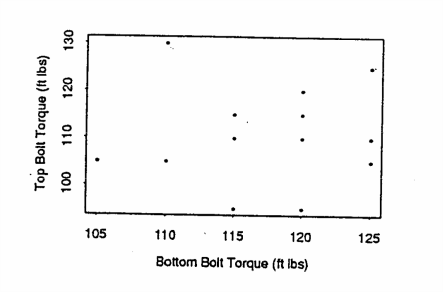
\includegraphics[width=0.6\textwidth]{./hw3_1_a.png}
			\end{center}
			{\color{red} There are no obvious patterns.}
		\item (5 points)
			{\color{red} The differences are -15, 0, -20, 0, -5, 0, -5, 0, -5,
			20, -25, -5, -10, -20, and 0.}

			\begin{center}
				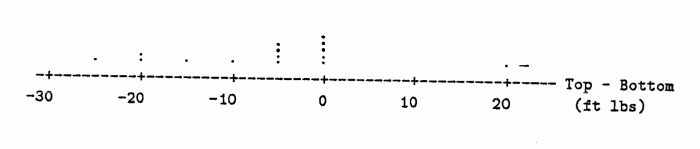
\includegraphics[width=0.6\textwidth]{./hw3_1_b.png}
			\end{center}

			{\color{red} 
			The dot diagram shows that most of the differences are
			zero or negative and ``truncated'' at zero. The
			exceptions is the 10th piece of equipment, which a
			difference of 20. This point does not fit in with the
			shape of the rest of the differences, so it is an
			outlier. Since most of the differences are zero or
			negative, the bottom bolt generally required more
			torque to loosen than the top bolt.
			}


	\end{enumerate}
	\clearpage
\item P. 114: 3
	\begin{enumerate}
		\item (5 points)
			\begin{center}
				{\color{red} \begin{tabular}{ccccc}
					$i$ & $\frac{i - .5}{10}$  & $Q_1(\frac{i -
					.5}{10})$  & $Q_2(\frac{i - .5}{10})$ &
					$Q_3(\frac{i - .5}{10})$\\ \hline
					1 & .05 & 74 & 82 & 78\\
					2 & .15 & 77 & 82 & 79 \\
					3 & .25 & 78 & 82 & 79 \\
					4 & .35 & 78 & 84 & 81\\
					5 & .45 & 78 & 84 & 82 \\
					6 & .55 & 80 & 85 & 82 \\
					7 & .65 & 81 & 85 & 82 \\
					8 & .75 & 84 & 85 & 83\\
					9 & .85 & 85 & 86 & 84\\
					10 & .95 & 87 & 87 & 85

			\end{tabular}
			
			\begin{tabular}{c|ccc}
				& $Q_1$ & Median & $Q_3$ \\ \hline
				Method 1 & 78 & $\frac{78 + 80}{2} = 79$ & 84\\
				Method 2 & 82 & $\frac{84 + 85}{2} = 84.5$ &
				85\\
				Method 3 & 79 & 82 & 83
			\end{tabular}
		}
		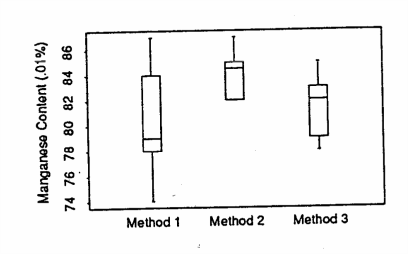
\includegraphics[width = 0.6\textwidth]{./hw3_2_a.png}
			\end{center}
		\item (4 points)
			{\color{red}
			Method 2 is the most precise, since it produces the
			least amount of spread. Method 3 is more precise than
			Method 1. Method 1 is the most accurate, since it comes
			to 80 on the average. Method 3 is more accurate than
			Method 2.
			}
		\item (3 points)
			These would be paired data. 10 specimens, 20
			measurements would provide a better comparison. To
			compare average under this plan, you would take
			differences for each of the specimens and look at the
			average of the 10 differences. Under the other plan,
			you would average measurements for 10 specimens for
			each method, and look at the differences between the
			averages. There will be less variability in the average
			of the differences than in the difference between
			averages, because of the pairing. Less variability
			results in a sharper comparison of the differences.
	\end{enumerate}
	\clearpage
\item P. 116: 8
	\begin{enumerate}
		\item (2 points)

			{\color{red}
				\begin{tabular}{ccccc}
					$i$ & $\frac{i - .5}{10}$ &
					$Q_1(\frac{i - .5}{10})$ & $Q_2(\frac{i
					- .5}{10})$ & $Q_{SN}(\frac{i -
				.5}{10})$ \\ \hline
				1 & .05 & 3.03 & 3.19 & -1.64 \\
				2 & .15 & 5.53 & 4.26 & -1.04 \\
				3 & .25 & 5.60 & 4.47 & -.67\\
				4 & .35 & 9.30 & 4.53 & -.39\\
				5 & .45 & 9.92 & 4.67 & -.13\\
				6 & .55 & 12.51 & 4.69 & .13\\
				7 & .65 & 12.95 & 5.78 & .39\\
				8 & .75 & 15.21 & 6.79 & .67\\
				9 & .85 & 16.04 & 9.37 & 1.04\\
				10 & .95 & 16.84 & 12.75 & 1.64
				\end{tabular}
			
				\vspace{2em}
			
			$Q(.84) = (.9) (16.04) + (.1)(15.21) = 15.957$}
		\item (2 points)
			{\color{red}
				(3.03, -1.64), (5.53, -1.04)
			}
		\item (5 points)
			\begin{center}
				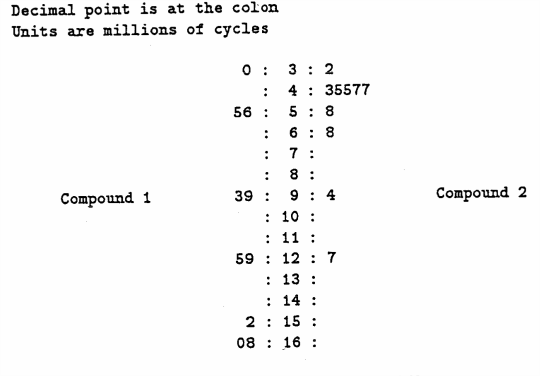
\includegraphics[width=0.6\textwidth]{./hw3_3_c.png}
			\end{center}
		\item (5 points)

			{\color{red}
				$\mathrm{Median}_1 = \frac{9.92 + 12.51}{2} =
				11.215,\, \mathrm{Median}_2 = \frac{4.67 +
				4.69}{2} = 4.68$.

				\begin{center}
					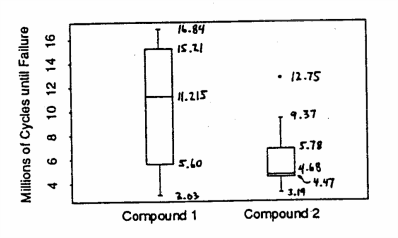
\includegraphics[width=0.6\textwidth]{./hw3_3_d.png}
				\end{center}
			}
		\item (2 points)
			{\color{red}
			$\bar{x}_1 = 10.693, s_1 = 4.819, \bar{x}_2 = 6.05, s_2
			= 2.915$.

			}
		\item (2 points)
			{\color{red}
		        The lifetimes of bearings mede with Compound 1 are
			generally longer than those made with Compound 2, but
			there is more variability in the lifetimes of bearings
			made with Compound 1 than in the lifetimes of those
			made with Compound 2.
			}

	\end{enumerate}
\item P. 119: 17
	
	\begin{enumerate}
		\item (5 points)
		
				\begin{minipage}{0.5\textwidth}
					{\color{red}
					\begin{tabular}{ccc}
						$i$ & $\frac{i - .5}{13}$ & $Q_A(\frac{i -
						.5}{13})$ \\ \hline
						1 & .04 & 79.97\\
						2 & .12 & 79.98\\
						3 & .19 & 80.00\\
						4 & .27 & 80.02\\
						5 & .35 & 80.02 \\		
						6 & .42 & 80.02\\
						7 & .50 & 80.03\\
						8 & .58 & 80.03\\
						9 & .65 & 80.03\\
						10 & .73 &  80.04\\
						11 & .81 & 80.04 \\
						12 & .88 & 80.04\\
						13 & .96 & 80.05
					\end{tabular}}
				\end{minipage}%
				\begin{minipage}{0.5\textwidth}
					{\color{red}
					\begin{tabular}{ccc}
						$i$ & $\frac{i - .5}{8}$ & $Q_B(\frac{i -
						.5}{8})$ \\ \hline
						1 & .06 & 79.94\\
						2 & .19 & 79.95\\
						3 & .31 & 79.97\\
						4 & .44 & 79.97\\
						5 & .56 & 79.97 \\		
						6 & .69 & 79.98\\
						7 & .81 & 80.02\\
						8 & .94 & 80.03\\
					\end{tabular}}
						\end{minipage}
		{\color{red}
		For Method A:
		
		$\mathrm{Median} = 80.03$\\
		$Q_1 = (\frac{6}{8})(80.02) + (\frac{2}{8})(80.00) = 80.015$\\
		$Q_3 = 80.04$
		
		For Method B:
		
		$\mathrm{Median} = 79.97$ \\
		$Q_1 = \frac{79.95 + 79.97}{2} = 79.96$ \\
		$Q_3 = \frac{79.98 + 80.02}{2} = 80.00$\\
		}
		
		\begin{center}
			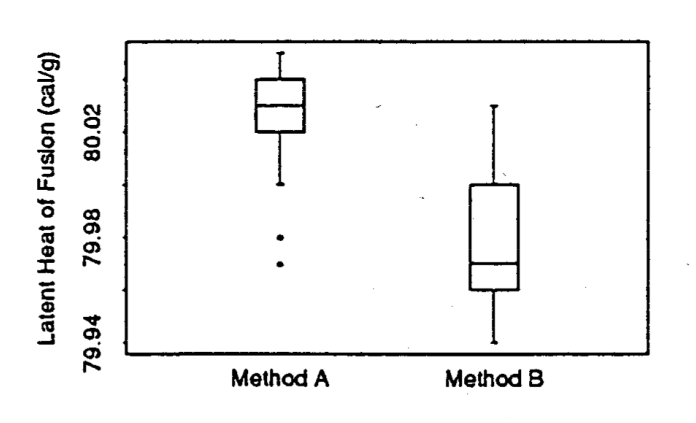
\includegraphics[width=0.6\textwidth]{./hw3_4_a.png}
		\end{center}
		
		{\color{red}
		There does not seem to be any important difference in the precisions of the two
		methods, but Method A generally produced larger values than Method B. Since
		there is some fixed, true, theoretical latent heat for the fusion of ice, at
		least one of the methods must be somewhat inaccurate.
		}
	\item (5 points)
		{\color{red}
			$\bar{x}_A = 80.021, s_A = .024, \bar{x}_B = 79.979, s_B =
		.031$. The sample standard deviations are similar, as reflected
		by the similar magnitudes of spread in the boxplots. $\bar{x}_A
		> \bar{x}_B$, as reflected by the location of the boxes on the
	boxplot.}
	\end{enumerate}


\end{enumerate}


%\newpage 
%\nocite{*}
%\bibliographystyle{plainnat} 
%\bibliography{}
\end{document}
